\documentclass[journal,onecolumn]{IEEEtran}

\makeatletter
\def\endthebibliography{%
	\def\@noitemerr{\@latex@warning{Empty `thebibliography' environment}}%
	\endlist
}
\makeatother
\usepackage{hyperref}
\usepackage{listings}
\usepackage{color}
\usepackage{float}
\usepackage{caption}
\usepackage{xcolor}

\usepackage{titlesec}
\titleformat{\section}    
       {\fontsize{16}{19}\bfseries}{\thesection}{1em}{}

\titleformat{\subsection}    
       {\fontsize{12}{17}\bfseries}{\thesubsection}{1em}{}

\titleformat{\subsubsection}    
       {\fontsize{12}{17}\bfseries\itshape}{\thesubsubsection}{1em}{}


\renewcommand{\thesection}{\Roman{section}} 
\renewcommand{\thesubsection}{\thesection.\Alph{subsection}}
\renewcommand{\thesubsubsection}{\thesubsection.\arabic{subsubsection}}


\usepackage[utf8]{inputenc}

% Default fixed font does not support bold face
\DeclareFixedFont{\ttb}{T1}{txtt}{bx}{n}{9} % for bold
\DeclareFixedFont{\ttm}{T1}{txtt}{m}{n}{9}  % for normal
\definecolor{deepblue}{rgb}{0,0,0.5}
\definecolor{deepred}{rgb}{0.6,0,0}
\definecolor{deepgreen}{rgb}{0,0.5,0}



% Python style for highlighting
\newcommand\pythonstyle{\lstset{
		language=Python,
		basicstyle=\ttm,
		morekeywords={self},              % Add keywords here
		keywordstyle=\ttb\color{deepblue},
		emph={MyClass,__init__},          % Custom highlighting
		emphstyle=\ttb\color{deepred},    % Custom highlighting style
		stringstyle=\color{deepgreen},
		frame=none,                         % Any extra options here
		showstringspaces=false,
		backgroundcolor = \color{lightgray}
}}

% Python environment
\lstnewenvironment{python}[1][]
{
	\pythonstyle
	\lstset{#1}
}
{}

\usepackage{graphicx}
\graphicspath{ {./Material/pictures/} }

\makeatletter
\renewenvironment{abstract}{%
    \if@twocolumn
      \section*{\abstractname}%
    \else %% <- here I've removed \small
      \begin{center}%
        {\bfseries \Large\abstractname\vspace{\z@}}%  %% <- here I've added \Large
      \end{center}%
      \quotation
    \fi}
    {\if@twocolumn\else\endquotation\fi}
\makeatother





% *** CITATION PACKAGES ***
%
%\usepackage{cite}
% cite.sty was written by Donald Arseneau
% V1.6 and later of IEEEtran pre-defines the format of the cite.sty package
% \cite{} output to follow that of the IEEE. Loading the cite package will
% result in citation numbers being automatically sorted and properly
% "compressed/ranged". e.g., [1], [9], [2], [7], [5], [6] without using
% cite.sty will become [1], [2], [5]--[7], [9] using cite.sty. cite.sty's
% \cite will automatically add leading space, if needed. Use cite.sty's
% noadjust option (cite.sty V3.8 and later) if you want to turn this off
% such as if a citation ever needs to be enclosed in parenthesis.
% cite.sty is already installed on most LaTeX systems. Be sure and use
% version 5.0 (2009-03-20) and later if using hyperref.sty.
% The latest version can be obtained at:
% http://www.ctan.org/pkg/cite
% The documentation is contained in the cite.sty file itself.
\hyphenation{op-tical net-works semi-conduc-tor}


\begin{document}
	%
	% paper title
	% Titles are generally capitalized except for words such as a, an, and, as,
	% at, but, by, for, in, nor, of, on, or, the, to and up, which are usually
	% not capitalized unless they are the first or last word of the title.
	% Linebreaks \\ can be used within to get better formatting as desired.
	% Do not put math or special symbols in the title.
	\title{Distance and Movement Measurement of an Object\\ based on Stereo Images}

	\author{Lennard~Rose,~5118054,~FHWS
		Moritz~Zeitler,~5118094,~FHWS% <-this % stops a space
	}
	% The paper headers
	\markboth{Seminar Smart Systems}%
	{Shell \MakeLowercase{\textit{et al.}}: Bare Demo of IEEEtran.cls for IEEE Journals}

	% make the title area
	\maketitle

	% As a general rule, do not put math, special symbols or citations
	% in the abstract or keywords.
	\begin{abstract}
   		\normalsize
		\noindent
		This paper explains how to compute distance to, and movement of an object with the means of stereo camera vision.
		Included is the whole workflow consisting of all steps that have to be made to get such a recognition to work. These steps are the hardware setup, all calibration steps, object detection, object tracking and the measurements of the values themselves.
	\end{abstract}


	% For peer review papers, you can put extra information on the cover
	% page as needed:
	% \ifCLASSOPTIONpeerreview
	% \begin{center} \bfseries EDICS Category: 3-BBND \end{center}
	% \fi
	%
	% For peerreview papers, this IEEEtran command inserts a page break and
	% creates the second title. It will be ignored for other modes.
	\IEEEpeerreviewmaketitle

	\section{Introduction}
\label{sec:einfuehrung}
\noindent
The human eye enables us to perceive our surroundings. Alongside with color and shape, it enables us to determine the position in relation to us and to each other. This is possible because a human being has two different point-of-views, the left and right eye. In this project, the so called Stereo-Vision will be applied with the means of a modern computer. To do this, a stereo camera setup is used to take photos/videos, create a depth map and try to compute the distance and movement of an object. The following chapters will describe this in a step by step fashion, starting with the basic theory behind it and the implementation afterwards.
\section{Prerequisites}
\noindent The initial idea was to run this Stereo-Vision on some kind of self driving vehicle, in our case a JetBot AI Kit\cite{jetbot_wiki}. This JetBot AI Kit is based on a NVIDIA Jetson Nano Developer Kit\cite{nvidia_jetson}. Mounted on this Bot is a the IMX219-83 Stereo Camera\cite{cam_wiki} of waveshare. After assessment of the provided resources and some in depth testing, the decision was made to not use the bot for running our applications, since it would impede development tremendously. This means all data used in the project was recorded using the bot, but all computation and programming was done on other machines. Obviously this means that the resulting pipeline should be deployable to the bot but there are some severe driver problems that stop this from happening.
\section{Stereoscopy}
\noindent
To visualize the idea behind stereoscopy, the human eye can be used as an intuitive example. Focusing on an object and alternately closing the eyes, the object will appear to be jumping right to left and vise versa. The closer the object, the farther the object will jump. With this information from the different viewpoints of our eyes, the brain is capable of perceiving depth. This is the whole concept behind stereoscopy simplified. Without this, it would be hard to impossible to guess the position of neighboring objects with the same appearance or do something simple as catching a ball out of the air.
When capturing a 3D object in an image, the objects gets projected from a 3D space to a 2D (planar) projection space. This is called the Planar Projection, the objects are losing all their depth information. The depth information can only be guessed by shadows our overlapping features. The question now is, how to get back the depth information from this 2D space, without the means of experience.
With 2 cameras, this is possible by comparing the left and the right image, called triangulation.
Finding an object on these two images can be done by using epipolar geometry and stereoscopy. This is basically to reduce the searchspace and not having to compare every pixel.

\begin{figure}[H]
	\centering
	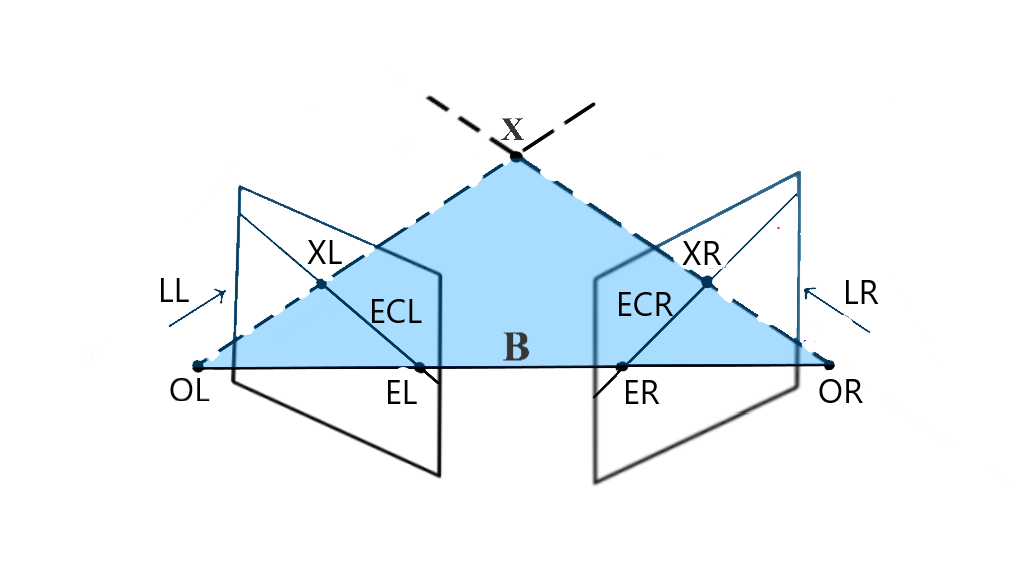
\includegraphics[scale=0.5]{epipolarGeometry.png}
	\captionsetup{justification=centering}
	\caption{Epipolar geometry}
\end{figure}
\noindent
This concept works by projecting the line {\bf LL} between the points {\bf OL}(left camera), {\bf XL}(projection of point {\bf X} in the left frame) and {\bf X}(being the target 3D point) as {\bf ECR} on our right picture, crossing the point {\bf XR}(projection of point {\bf X} in the right frame). The same on the left picture, project the line {\bf LR} between the points {\bf OR}(right camera), {\bf XR} and {\bf X}, crossing the point {\bf XL} as {\bf ECL}. The centers of both cameras get also project to there significant other frame.
With this, the searchspace got reduced of a corresponding point to compute our disparity from to a single line, {\bf ECL} respectively {\bf ECR} (this is called an epipolar constraint). {\bf EL} and {\bf ER} is the projection of one camera onto its significant other cameras pov. These points are called epipoles. Together with {\bf LL} and {\bf LR} this baseline forms the epipolar plane (blue in figure 5). All this information can be represented by the Fundamental matrix of the image, which can be calculated with the projected points and the projection matrices of the cameras. Further mathematical description can be found in the book \emph{Multiple View Geometry in Computer Vision}\cite{hartley_zisserman_2004}, but won't be discussed any further at this point.

\section{Workflow}
\noindent
This chapter contains a detailed theoretical and practical description of each individual step in the workflow.
\subsection{Stereo Camera Calibration}
\noindent
Cameras are projecting a three dimensional object to a two dimensional image. This projection is never alone determined by the original object, but also by all parameters of the used camera. These you can separate in two groups, external and internal. External parameters are the camera orientation in different planes. Internal parameters are determined by the cameras internal characteristics.
\begin{figure}[H]
	\centering
	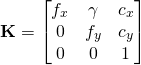
\includegraphics[scale=0.8]{intrinsicMatrix.png}
	\captionsetup{justification=centering}
	\caption{Intrinsic Matrix}
\end{figure}
\noindent
These internal parameters are represented as an upper triangular matrix K. This matrix has the values fx and fy as the x and y focal lengths. cx and cy as the x and y coordinates of the optical center in the image plane. Gamma is the distortion between the axes, this value is replaced by a "0" in OpenCV´s calibration function.\newline
\begin{figure}[H]
	\centering
	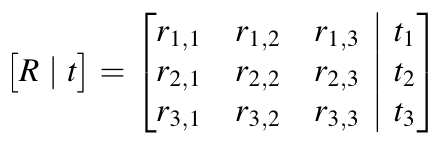
\includegraphics[scale=0.4]{extrinsicMatrix.png}
	\captionsetup{justification=centering}
	\caption{Extrinsic Matrix}
\end{figure}
\noindent
The external parameters are represented by an 3x3 rotation matrix, that indicates the rotation bias of the camera. Combined with an 3x1 translation vector, which describes the position of the world coordinates origin in the camera coordinate system.\newline
\begin{figure}[H]
	\centering
	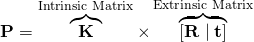
\includegraphics[scale=0.7]{projectionMatrix.png}
	\captionsetup{justification=centering}
	\caption{Projection Matrix}
\end{figure}
\noindent
Together these form the 3x4 Projection Matrix. This matrix and the real world coordinates of our point is used to calculate the image coordinates of the 2D projection. Calibration does nothing else than alter these matrices so our 2D projection matches the 3D object in the real world. This is usually done by giving the calibrating program/ function a set of 2D images with known 3D coordinates. 
This Calibration consists of two steps removing of Distortion as well as rectifying the images\cite{ImageRectification}. \newline
\subsubsection{Distortion}
\noindent
A camera lens always has some kind of curvature. This curvature is also visible in an image taken with this lens. This is called distortion. There are many different types of distortion which can be seen in the next figure.
\begin{figure}[H]
	\centering
	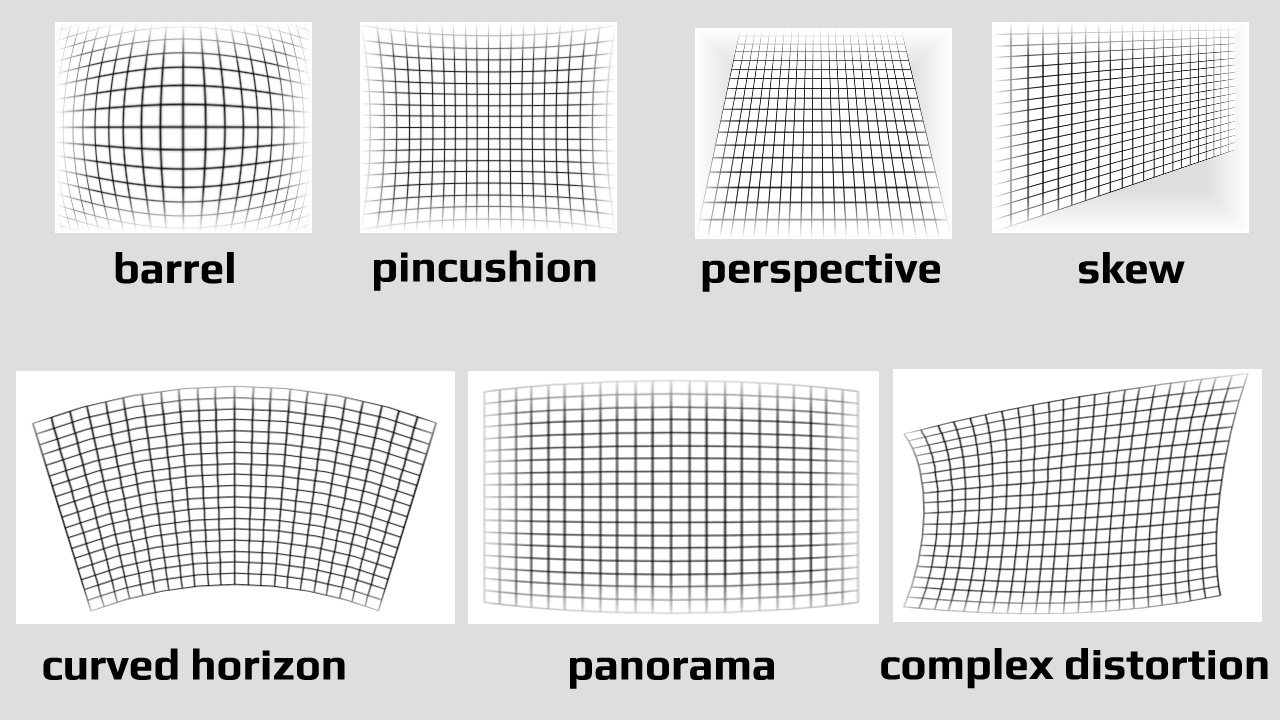
\includegraphics[scale=0.3]{distortion.jpg}
	\captionsetup{justification=centering}
	\caption{Different types of distortion}
\end{figure}
\noindent
To remove this distortion pictures of a chessboard were taken. OpenCV, the package used to do all calibration steps, can easily detect key points using this chessboard pattern. This is based on the big difference in pixel values between white and black. In combination with the size of the squares as well as the amount of the squares, OpenCV is able to create a calibration matrix removing the distortion.\newline
A very important part is to be very precise while taking the calibration pictures. To get a good result you need to take calibration photos from all parts and angles of the cameras perspective.\newline
The python implementation looks like the following: \newline
First of all  the input picture was converted to grayscale and passed to a detection function for chessboard corners.
\begin{python}
ret, corners = cv2.findCirclesGrid(inputImage, (chessboardColumns, chessboardRows), None)
\end{python}
The input is the chessboard picture, columns of the chessboard, rows of the chessboard and an output array not further used.
This function returns whether a chessboard got detected and if so the 2D points of the chessboard corners. If the detection was successful the returned points get even more refined using:
\begin{python}
cv2.cornerSubPix(inputImage, corners, (11, 11), (-1, -1), criteria)
\end{python}
The 'cornerSubPix' of openCV refines the corner locations \cite{forstner} of the checkboard.
All results of the previous steps are saved in a list, which caches them for future use. With these lists a single camera can be calibrated :
\begin{python}
ret, mtx, dist, rvecs, tvecs = cv2.calibrateCamera(object_pts, img_pts, img.shape[::-1], None, 
											None)
\end{python}
Passing these points as well as the shape of the image into the calibrate Camera function delivers the intrinsic and extrinsic parameter.
These parameters are stored inside the mtx variable. Also the overall RMS re-projection error in ret and the distortion coefficients are returned. Rvecs\cite{DBLP} and tvecs are rotational and translation vectors, which aren't used in this system and won't be described further.
On a high level openCV executes the global Levenberg-Marquardt optimization algorithm to minimize the reprojection error, that is, the total sum of squared distances between the observed feature points imagePoints and the projected (using the current estimates for camera parameters and the poses) object points objectPoints\cite{calibrateCamera}.
With these matrices a new optimal matrix based on these parameters can now be computed.
\begin{python}
h, w = img.shape[:2]
new_mtx, roi = cv2.getOptimalNewCameraMatrix(mtx, dist, (w, h), 1, (w, h))
\end{python}
As a result the function returns a new optimal intrinsic camera matrix. The function also returns a valid pixel region which outlines a region of all-good-pixels in the undistorted image. These matrices and results will be later used to undistort and rectify images coming from our camera for better results while computing the disparity and depth map.



\subsubsection{Rectification}
\noindent
With image rectification, the goal is to project the two different images taken by the camera onto a common image plane. This process ensure that the individual horizontal pixel-lines of both images are on the same level. This means the epipolarlines are calibrated to be exactly horizontal, which helps finding the correspondence of a point in both of the stereo pictures by reducing the searchspace to a horizontal line.
For this step the previous calibration matrices for both of our cameras as well as pictures from both cameras are needed at a similar time containing the chessboard to compute the rectification. This computes us the following matrices and vectors:
\begin{enumerate}
	\item essential matrix
	\item rotational matrix
	\item translation vector (previously described as extrinsic matrix) %wo? nochmal gucken, wäre mir jetzt nicht aufgefallen
\end{enumerate}

\begin{python}
retS, new_mtxL, distL, new_mtxR, distR, Rot, Trns, Emat, Fmat = cv2.stereoCalibrate(obj_pts,
 										img_ptsL,
 										img_ptsR,
 										mtxL, distL,
 										mtxR, distR,
 										imgR.shape[::-1],
 										criteria_stereo,
 										flags)
\end{python}
The function can also compute the full calibration for each of the cameras but isn't recommended to do so due to the high dimensionality of the parameter space and noise in the input data\cite{stereoCalibrate}. Because of this the individual calibration is done beforehand and gets supplied as an input.
These matrices allows computation of a coordinate representation of a 3D point in one of the cameras using the result matrices as well as the one of the individual camera matrices.
Similarly to calibrateCamera, the function minimizes the total re-projection error for all the points in all the available views from both cameras. The function returns the final value of the re-projection error.
Now the goal is to rectify these cameras using stereoRectify:
\begin{python}
rect_l, rect_r, proj_mat_l, proj_mat_r, Q, roiL, roiR = cv2.stereoRectify(new_mtxL, 
 										distL, 
 										new_mtxR, 
 										distR,
 										imgL.shape[::-1],
  										Rot, Trns,
  										rectify_scale,
 										(0, 0))
\end{python}
Once again all previous results are input for the function. The function results in two rectification transform matrices, which transfer points from unrectified camera's coordinate system to points in the rectified camera's coordinate system.

\subsection{Disparity Map}
\noindent
Disparity is usually computed as a shift of an image feature when viewed in the right/left image. For example, a single point that appears at the x coordinate k (measured in pixels) in the left image may be present at the k coordinate k minus 3 in the right image. This would result in a disparity value of 3 in pixels. These disparity values are the base for the later computation of the depth map.
This can be done using specific algorithms, in this case the Block Matching Algorithm is used.
\begin{figure}[H]
	\centering
	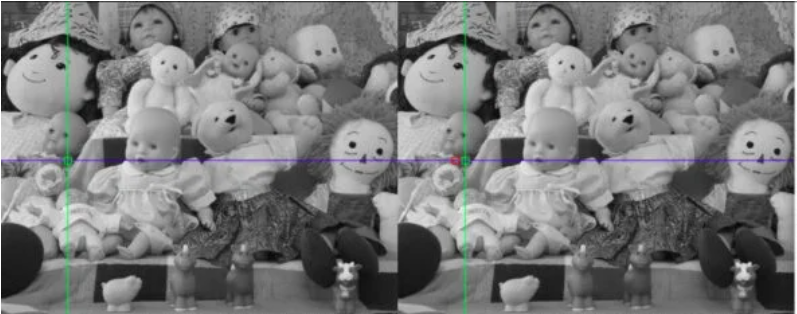
\includegraphics[scale=0.65]{bma.png}
	\captionsetup{justification=centering}
	\caption{Visualization of the Block Matching Algorithm working on input and output image}
\end{figure}
\noindent
The above figure displays the method the algorithm implements. Input is one pixel, or in this case a small window(box) of pixels, which makes the algorithm more resilient. With the input the algorithm searches the most similar neighbor in the corresponding stereo picture. In this case the left image is the input, with the red square as the search window. The algorithm searches for its corresponding window on the right picture. The best match is visualized by the red window, the coordinates of the original box in yellow. The green line indicates the epipolar constraint.
This can be done in with different metrics, for example absolute or normalized differences. The algorithm searches for the least differences to determine correspondence. However, the algorithm tends to find multiple pairs of corresponding points due to repeating textures or similar occurrences, in this case this would be most of the boxes brown surface, the wall or the floor.
In Python the algorithm is implemented as a class which needs to be instantiated. To be more precise, the implementation used in this project is slightly more advanced\cite{SGBM} but follows the same principle.
\begin{python}
stereo = cv2.StereoSGBM_create(minDisparity=min_disp,
			       numDisparities=num_disp,
			       blockSize=window_size,
			       uniquenessRatio=10,
			       speckleWindowSize=100,
			       speckleRange=32,
			       disp12MaxDiff=5,
			       P1=8*3*window_size**2,
			       P2=32*3*window_size**2)
\end{python}
Important are the different options supplied to the SGBM class. The block size parameter supplies the window size for the algorithm. The disparity amount, which has a minimum and a maximum, specifies at which range a disparity match is acceptable. Speckleand P1 and P2 are filtering algorithms to smooth the output\cite{stereoSGBM}, again further explanation will be skipped.
To improve those parameters, an user interface was build to change the values on the fly.
\begin{figure}[H]
	\centering
	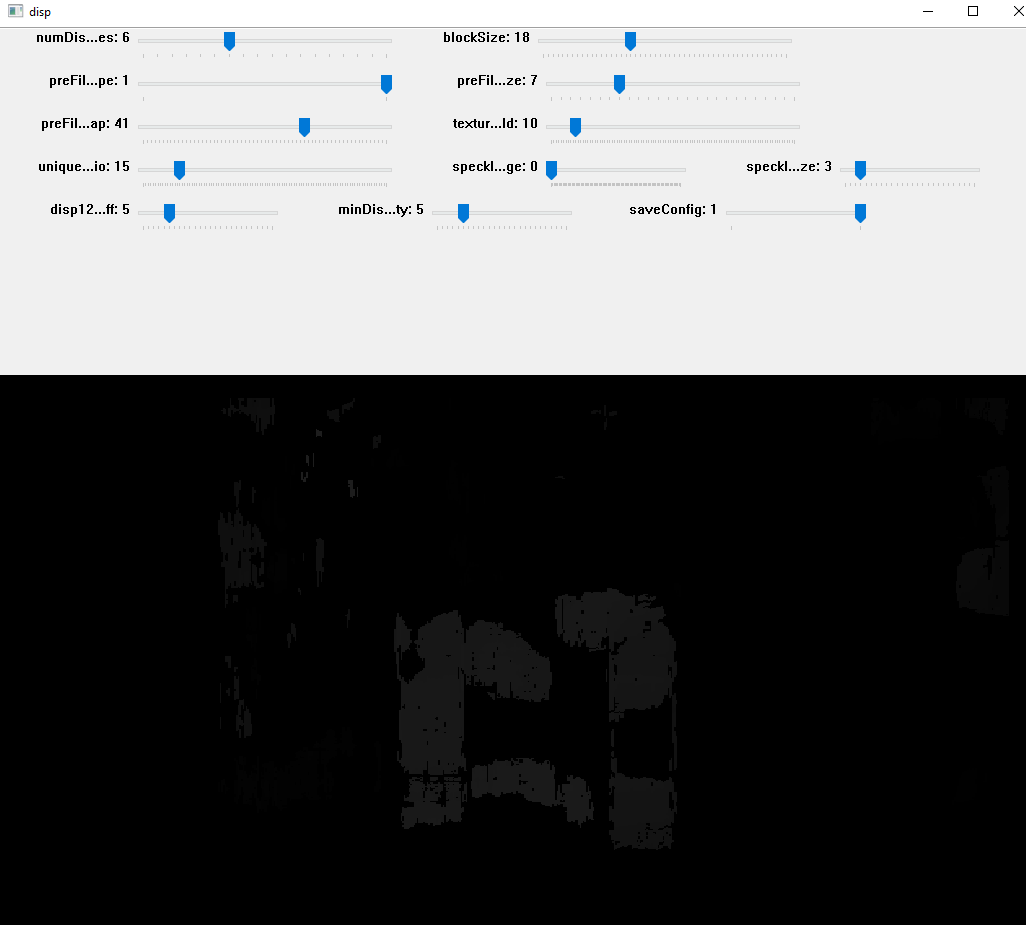
\includegraphics[scale=0.5]{calibrateUI.png}
	\label{UI}
	\captionsetup{justification=centering}
	\caption{UI for calibrating all parameters of the Block Matching Algorithm}
\end{figure}
\noindent
In the UI are many different parameters to tune. Also there is the option to save the parameters. It isn't currently possible to use a button in openCV thus there is a slider which produces a config.json.The result can look something like Figure 8.
\begin{figure}[H]
	\centering
	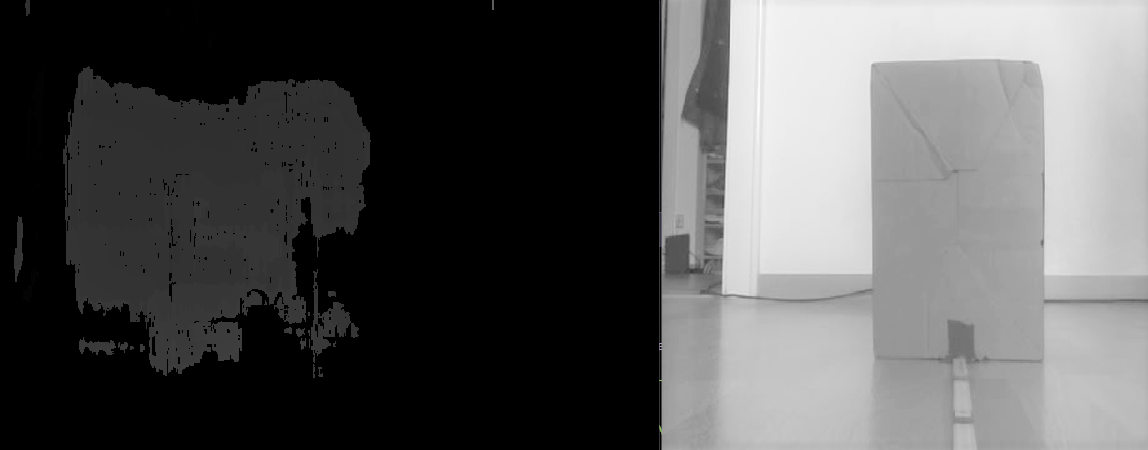
\includegraphics[scale=0.5]{disparityMap.png}
	\captionsetup{justification=centering}
	\caption{Resulting Disparity Map after calibration without filtering on the left, greyscale left cameras image on the right}
\end{figure}

\subsection{Depth Map}
\noindent
\noindent At this point there are two different options to compute a depth value from the previously created disparity map. The first one being the usage of the openCV function 'reprojectImageTo3D', which takes the disparity map as well as the Q matrix computed  previously during the rectification process to compute a depth map.
Alternatively computation of the distance with the inverse disparity-value is possible. The relation between depth and disparity is non-linear, but by using the inverse this relation becomes linear. 
\begin{figure}[H]
	\centering
	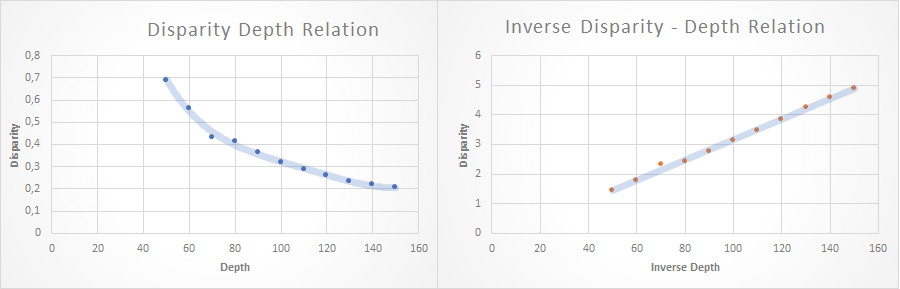
\includegraphics[scale=0.5]{ratios.png}
	\captionsetup{justification=centering}
	\caption{Relation between Depth and Disparity(left) and Inverse Disparity(right)}
\end{figure}
\noindent The equation for this is the following: 
\begin{equation}
	Distance = \frac{M}{Disparity}
\end{equation}
\noindent With M being the product of the focal length f and the baseline B of the camera. \newline
In this practical scenario, the assumption was made that some of these values may have a small error. This might be because the disparity values are not as exact as expected, or because the camera has some internal calibration or construction issues. Because of these issues, the  M value isn't just computed. Simirlaly to the UI used to find the optimal parameters for the Blockmatching Algorithm ~\ref{UI}, the M parameter gets sort of calibrated as well. 
\subsubsection{Measurement}
For testing purposes the initial idea is an event based system. On double-click an openCV event gets triggered, containing a x and y position of the mouse click. These values get enhanced to a window, all disparity values in this window get added up to compute an average. With this basic function computing the distance can be encapsulated . This results in following precision:
\begin{table}[H]
	\begin{tabular}{|l|l|}
		\hline
		actual distance & computed distance \\ \hline
		0.5             & 0.5               \\ \hline
		0.5             & 0.5               \\ \hline
		0.6             & 0.61              \\ \hline
		0.6             & 0.6               \\ \hline
		1.2             & 1.18              \\ \hline
		1.2             & 1.18              \\ \hline
		1.3             & 1.28              \\ \hline
		1.3             & 1.31              \\ \hline
		1.4             & 1.44              \\ \hline
		1.4             & 1.42              \\ \hline
	\end{tabular}
\end{table}
\noindent The mean squared error of these observations is 0.00034. The closer the value to 0 the better the result, meaning that the computed distance is extremely good. But this needs to be put into perspective, meaning this test was performed under laboratory conditions which should result in this kinda of perfection.
\begin{figure}[H]
	\centering
	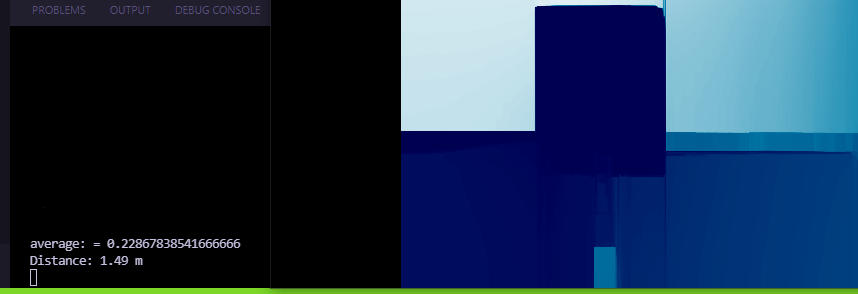
\includegraphics[scale=0.5]{distanceCalcRegression.png}
	\captionsetup{justification=centering}
	\caption{Depth map calculated with blue color filter and a computed distance based on a regression function}
\end{figure}

\subsection{Object Detection}
\noindent For object detection the first idea was to track large appearances on the disparity map sorted by their calculated depth, beginning with the nearest. Due to the disparity map being an unprecise projection of the real picture, this algorithm ended up detecting only unusable patterns:
\begin{figure}[H]
	\centering
	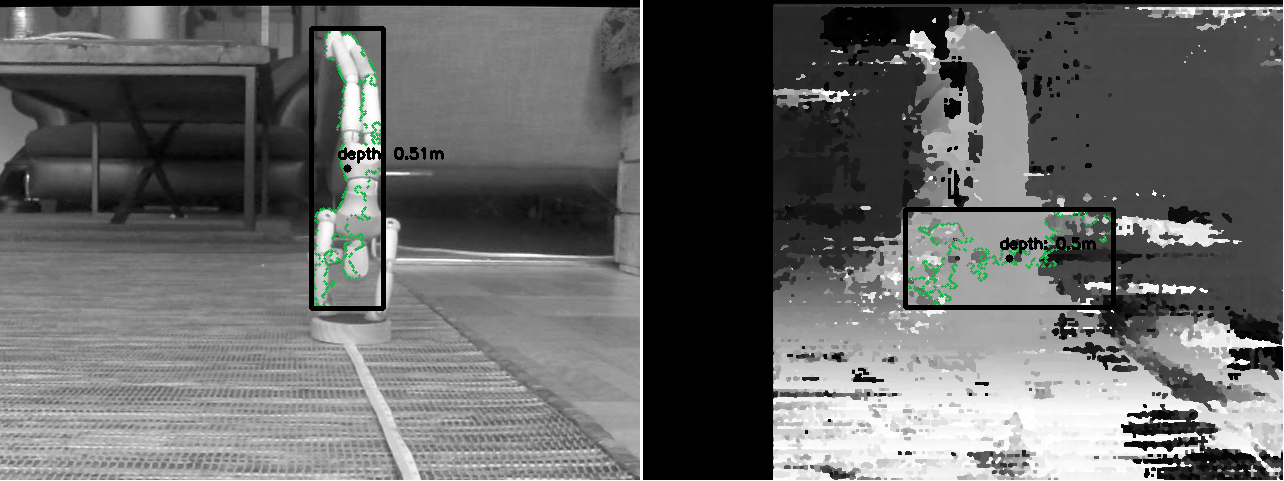
\includegraphics[scale=0.5]{handstand_comparison.png}
	\label{tracking}
	\captionsetup{justification=centering}
	\caption{Left: Detection on original picture Right: Detection on disparity picture }
\end{figure}
\noindent To solvee this problem the original grayscale picture of one of the cameras was used to detect the objects. This was done by creating a mask that substrackts the unmoving areas of the picture, leaving only the targeted object. This was done by using the following openCV function:
\begin{python}
back_sub = cv2.createBackgroundSubtractorMOG2(history=500, varThreshold=25, detectShadows=False)
\end{python}
\noindent The  'createBackgroundSubtractorMOG2' function works by comparing a history of frames and declaring its unchanged pixels as background. The result is a mask only containing the potential objects that should be tracked. On this, some filtering is performed:
\begin{python}
# Close dark gaps in foreground objects
mask = cv2.morphologyEx(mask, cv2.MORPH_CLOSE, kernel)
# Remove noise
mask = cv2.medianBlur(mask, 5) 
# Threshold the image to make it either black or white
_, mask = cv2.threshold(mask,127,255,cv2.THRESH_BINARY)
\end{python}
\noindent After preparing the images, applying openCVs findContours() function, the objects get outlined.
\begin{python}
contours, hierarchy = cv2.findContours(mask,cv2.RETR_TREE,cv2.CHAIN_APPROX_SIMPLE)[-2:]
\end{python}
RETR\_TREE computes a full hirarchy list for shapes inside other shapes. CHAIN\_APPROX\_SIMPLE on the other hand removes all redundant points of the contourlines, leaving only the necessary minimum.
\begin{python}
x,y,w,h = cv2.boundingRect(cnt)
cv2.rectangle(grayL,(x,y),(x+w,y+h),(0,255,0),3)
# Draw circle in the center of the bounding box
centerpoint_x = x + int(w/2)
centerpoint_y = y + int(h/2)
cv2.circle(grayL,(centerpoint_x, centerpoint_y),4,(0,255,0),-1)
\end{python}
\noindent Next step is to draw a bounding rectangle around the object and a point in its center. This points disparity value is used for the distance calculation. This might lead to error, if the object is for example ring-shaped, but taking the average of all the objects disparity-values led to big inacurracies. A way to optimize this was not further pursued. \newline
This rectangle and point were also used to prevent jumps caused by the inacurracy of the contour-algorithm, as described in the next section. 

\subsection{Object Tracking and Direction}
\begin{figure}[H]
	\centering
	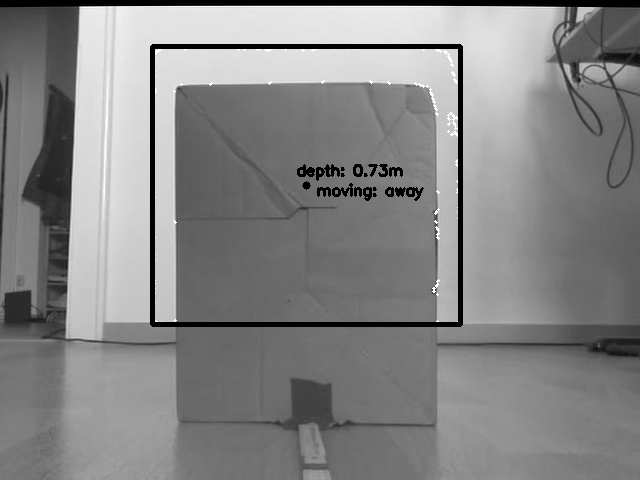
\includegraphics[scale=0.5]{box_direction.png}
	\captionsetup{justification=centering}
	\caption{Object with movement direction}
\end{figure}
\noindent The detected Objects were tracked by saving their coordinates, as well as their distance to an array. Only Objects with their centerpoint within the rectangle-coordinates of the previous frames object, as well as the changed depth within a range were taken into consideration, otherwise skipped. The centerpoints coordinates and depth were then compared to the average of the last 3 points and its movement on the 3 axis determined as shown in the next table: 
\begin{table}[H]
	\begin{tabular}{|l|l|}
		\hline
		condition & direction \\ \hline
		 current centerpoint x smaller than average of the last centerpoints x             & left               \\ \hline
		 current centerpoint x bigger than average of the last centerpoints x              & right               \\ \hline
		 current centerpoint y smaller than average of the last centerpoints y             & up               \\ \hline
		 current centerpoint y bigger than average of the last centerpoints y             & down             \\ \hline
		 current centerpoint z smaller than average of the last centerpoints z             & closer             \\ \hline
		 current centerpoint z bigger than average of the last centerpoints z              & away              \\ \hline
	\end{tabular}
\end{table}
\subsubsection{Measurement}
\noindent With the test video tracking a box moving away from us, an accuracy of 70,5\% was archieved with this simple implementation. Almost all wrong calculated directions were caused by incorrect disparity-values, "jumping" arround the correct value. For example with the box standing 80cm away from the camera, the values tended to jump between 79 and 81cm, causing false directions. 

 
\section{Conclusion}
\noindent The most important conclusion of this study is quite sobering. With the experience gained from working with the system, there are way too many factors that influence the result. Even more important those factors or variables are not always controllable. This means from time to time, results from some functions are more or less arbitrary. Especially the calibration of the stereo cameras is quite a difficult task. Most of the time the result of openCV calibration, meaning removing of Distortion as well as rectifying images, isn't comprehensible. A big variable are the pictures, and their quality, as a consequence this means the camera used is quite important. In our case the cameras are designed for this purpose, but this doesn't mean the cameras don't have problems. Basically the calibration process was done by try and error. This means the calibration is not as easy as most documentations suggest. By this a the following algorithms, for example computation of distance, are inferred by this, lets call it blur. \newline
If those problems are left aside the result for distance as well as speed are quite satisfying. With a better setup that doesn't depend as much on calibration, for example usage of a Intel RealSense camera could enhance the result enormously. And almost as important, would ease up development since the camera modul for JetBot in combination with the nVidia Jetson Nano development board does also provide some problems which won't be discussed at this point. \newline
As a final conclusion, on a theoretical level, the initial problem doesn't sound really super complex. But once we factor in the practical part the difficulty level rises significantly. All in all this means the result of this study is quite satisfying once it's viewed from an objective standpoint.
\appendices

% can use a bibliography generated by BibTeX as a .bbl file
% BibTeX documentation can be easily obtained at:
% http://mirror.ctan.org/biblio/bibtex/contrib/doc/
% The IEEEtran BibTeX style support page is at:
% http://www.michaelshell.org/tex/ieeetran/bibtex/
%\bibliographystyle{IEEEtran}
% argument is your BibTeX string definitions and bibliography database(s)
\bibliography{bibtex/bib/IEEEabrv.bib,bibtex/bib/IEEEexample.bib}{}
\bibliographystyle{IEEEtran}

%
% <OR> manually copy in the resultant .bbl file
% set second argument of \begin to the number of references
% (used to reserve space for the reference number labels box)

\end{document}